% Hamad Medical Corporation
% Georges Younes

\appendix%

\chapter{Appendix}
Test for acronyms and nomenclatures

\gls{usb} $\gls{c}^2$

\chapter{Collision Dectection API}\label{apn:collision_detection_api}

\chapter{RARP Steps}\label{apn:rarp_steps}

\chapter{Evaluation Questionnaire}\label{apn:evaluation_questionnaire}
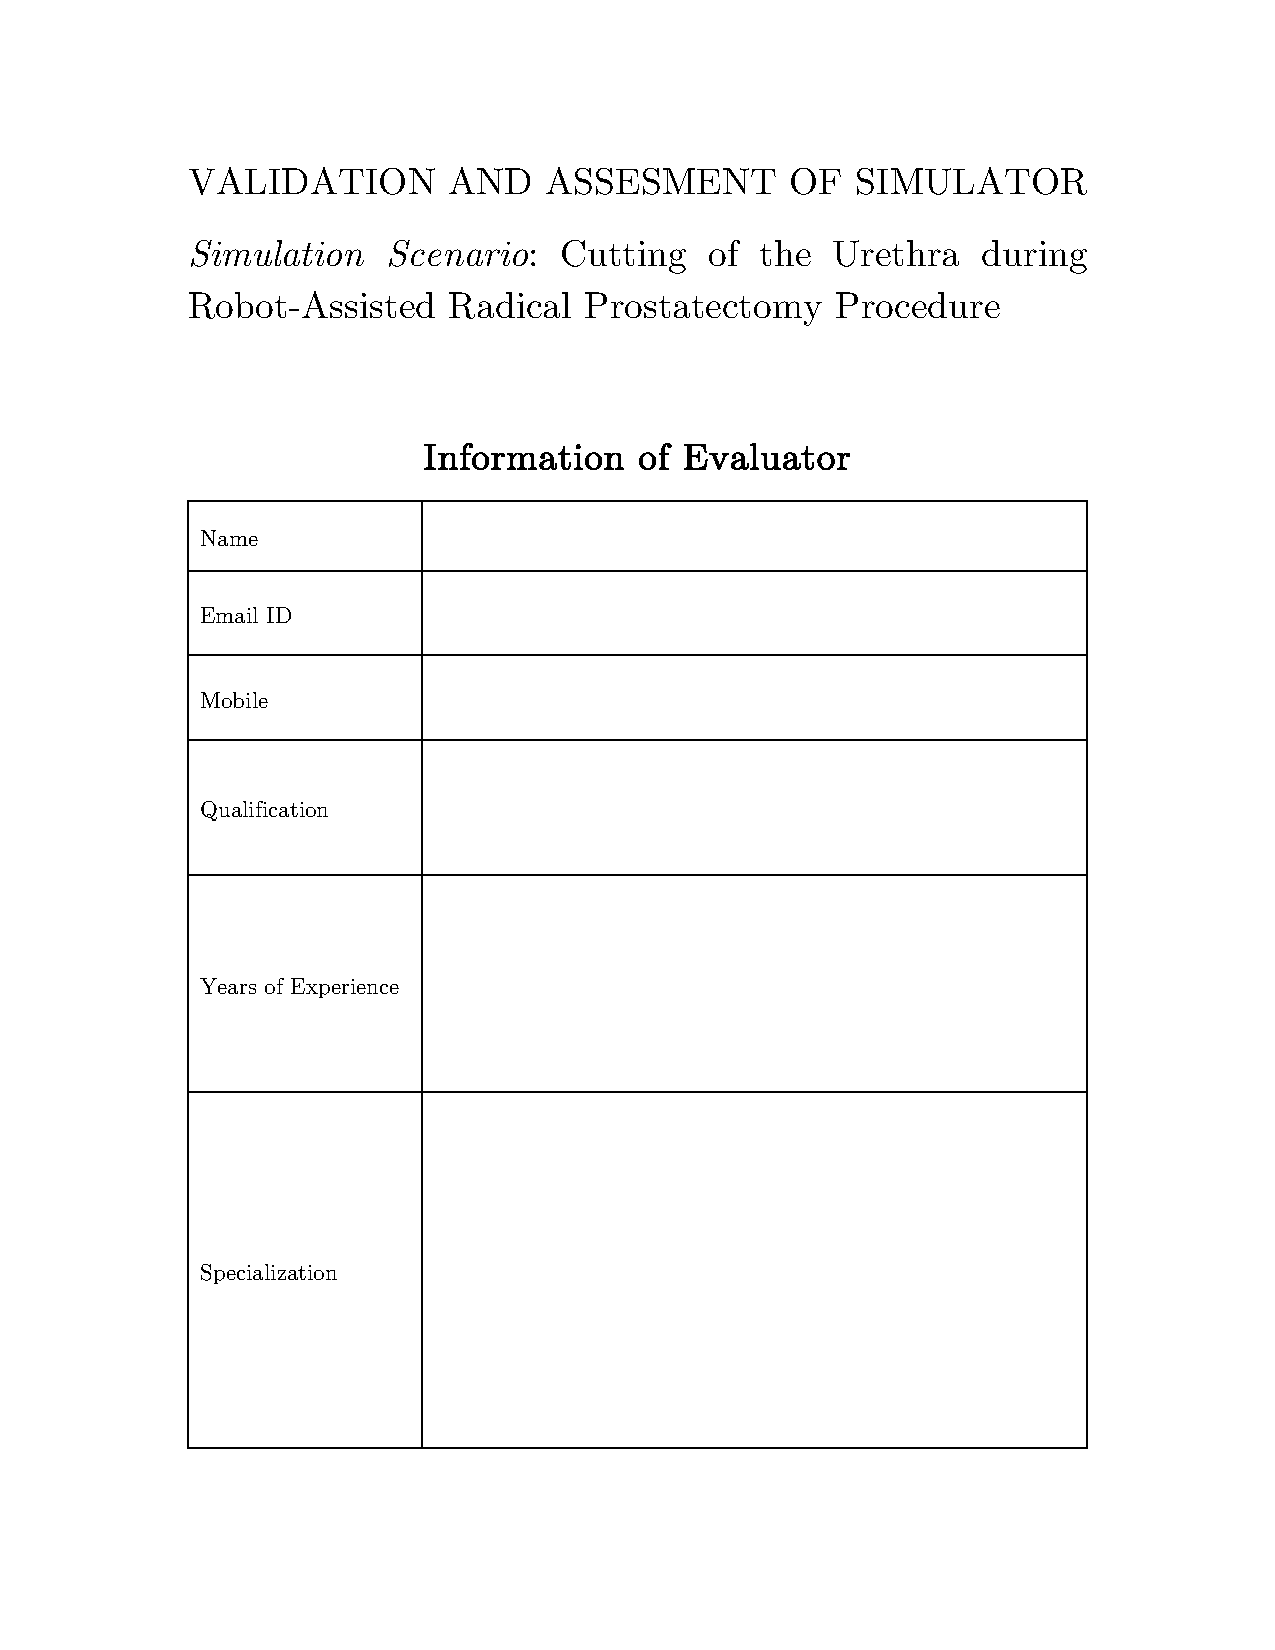
\includepdf[pages=-,scale=0.95,pagecommand={}]{documents/validation/questionnaire.pdf}

\chapter{Logging of Metrics}\label{apn:logging_metrics}
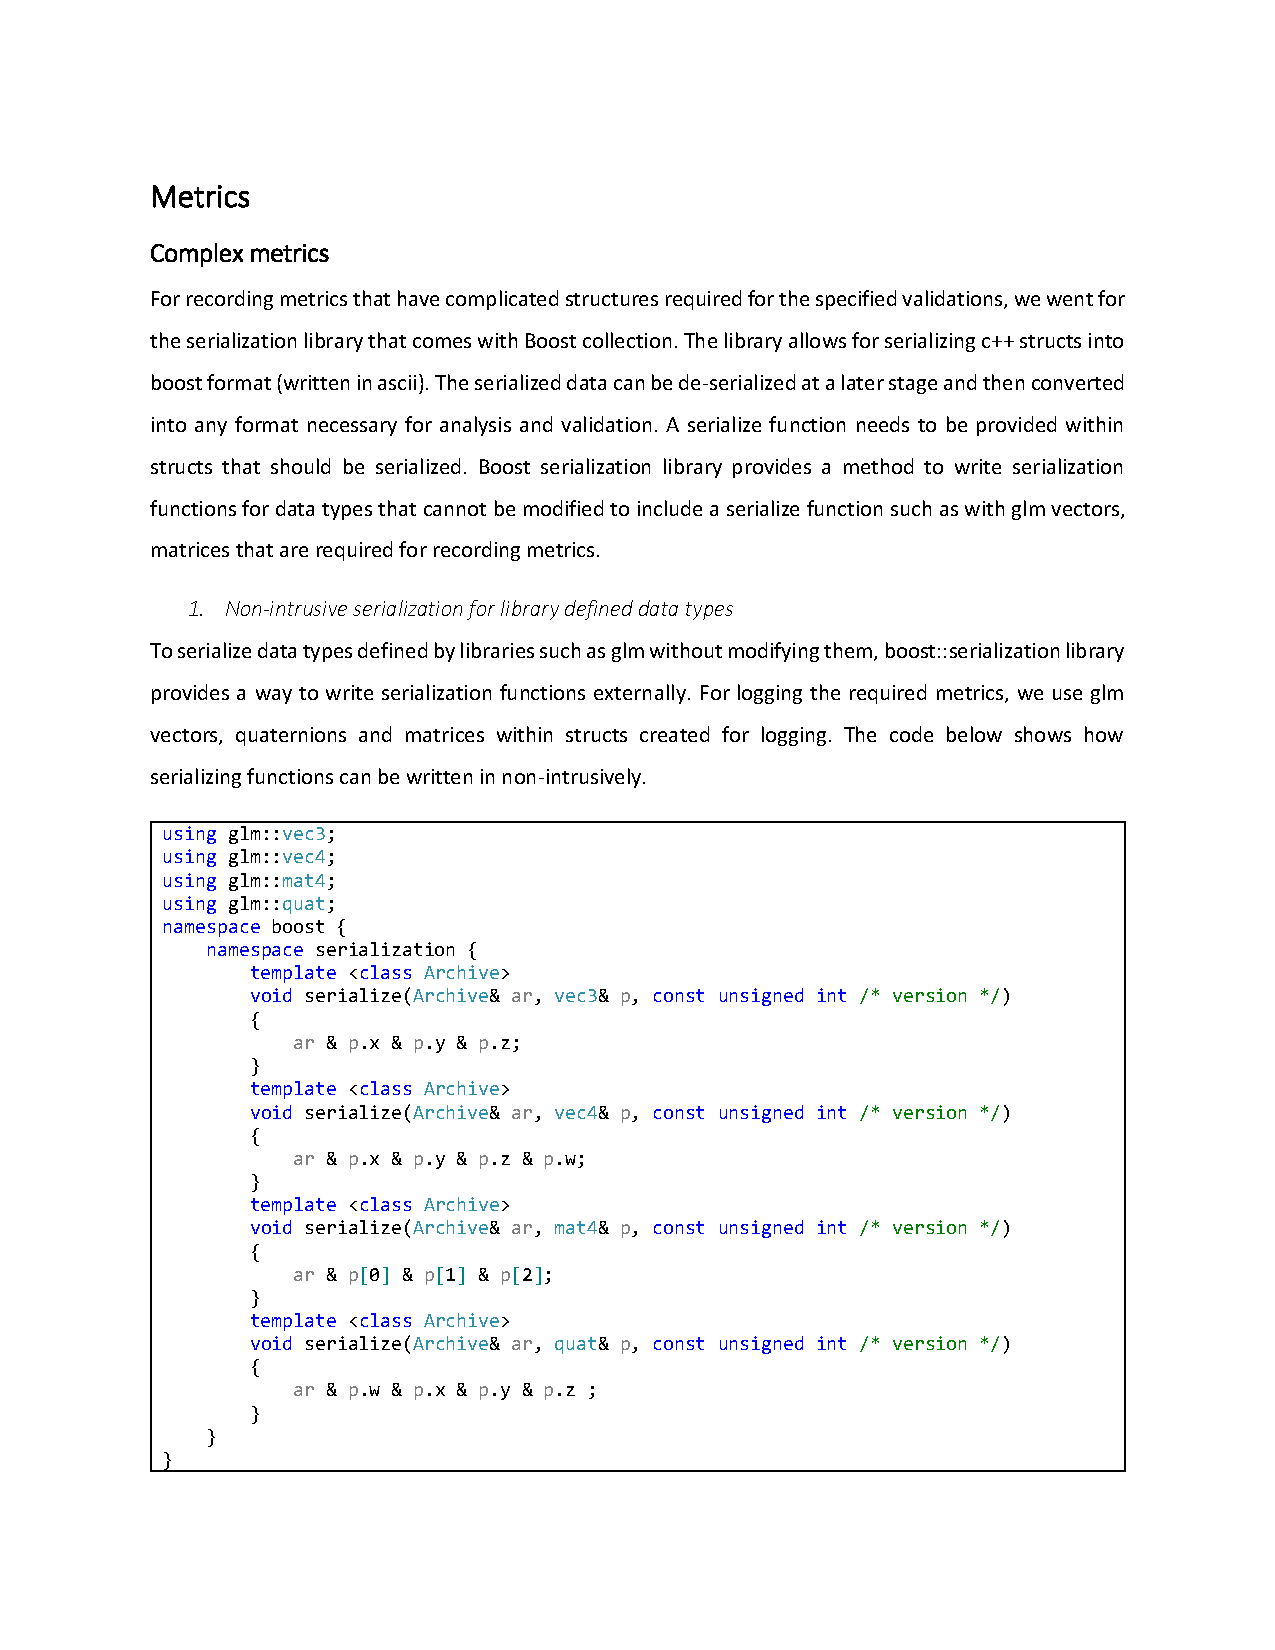
\includepdf[pages=-,scale=0.95,pagecommand={}]{documents/validation/logging.pdf}

\chapter{Surgeon Responses}\label{apn:surgeon_responses}
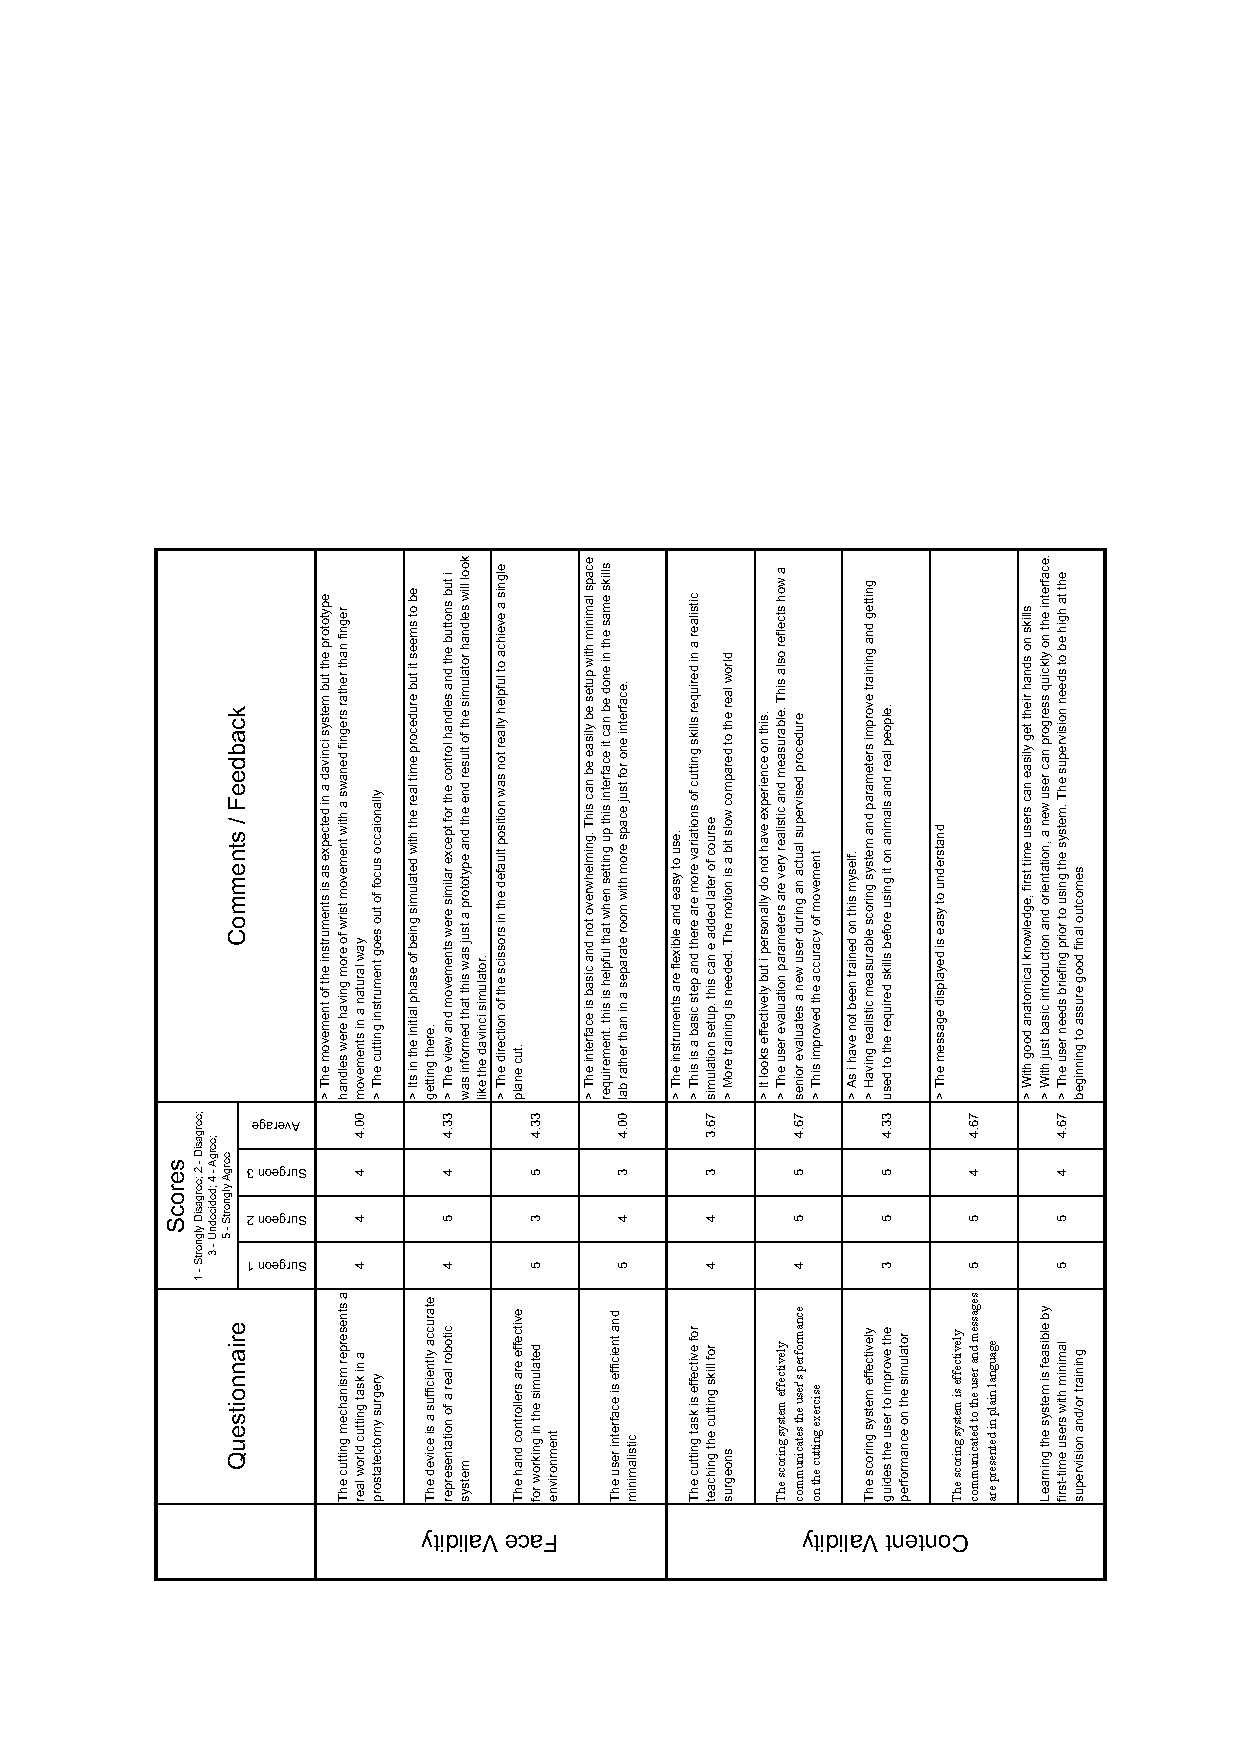
\includepdf[pages=-,scale=1.50,pagecommand={},angle=270,offset=3.5cm 0cm]{documents/validation/surgeon_responses.pdf}

%%% https://stackoverflow.com/questions/2034766/when-using-pdfpages-in-latex-how-to-avoid-page-breaks-before-the-first-page
%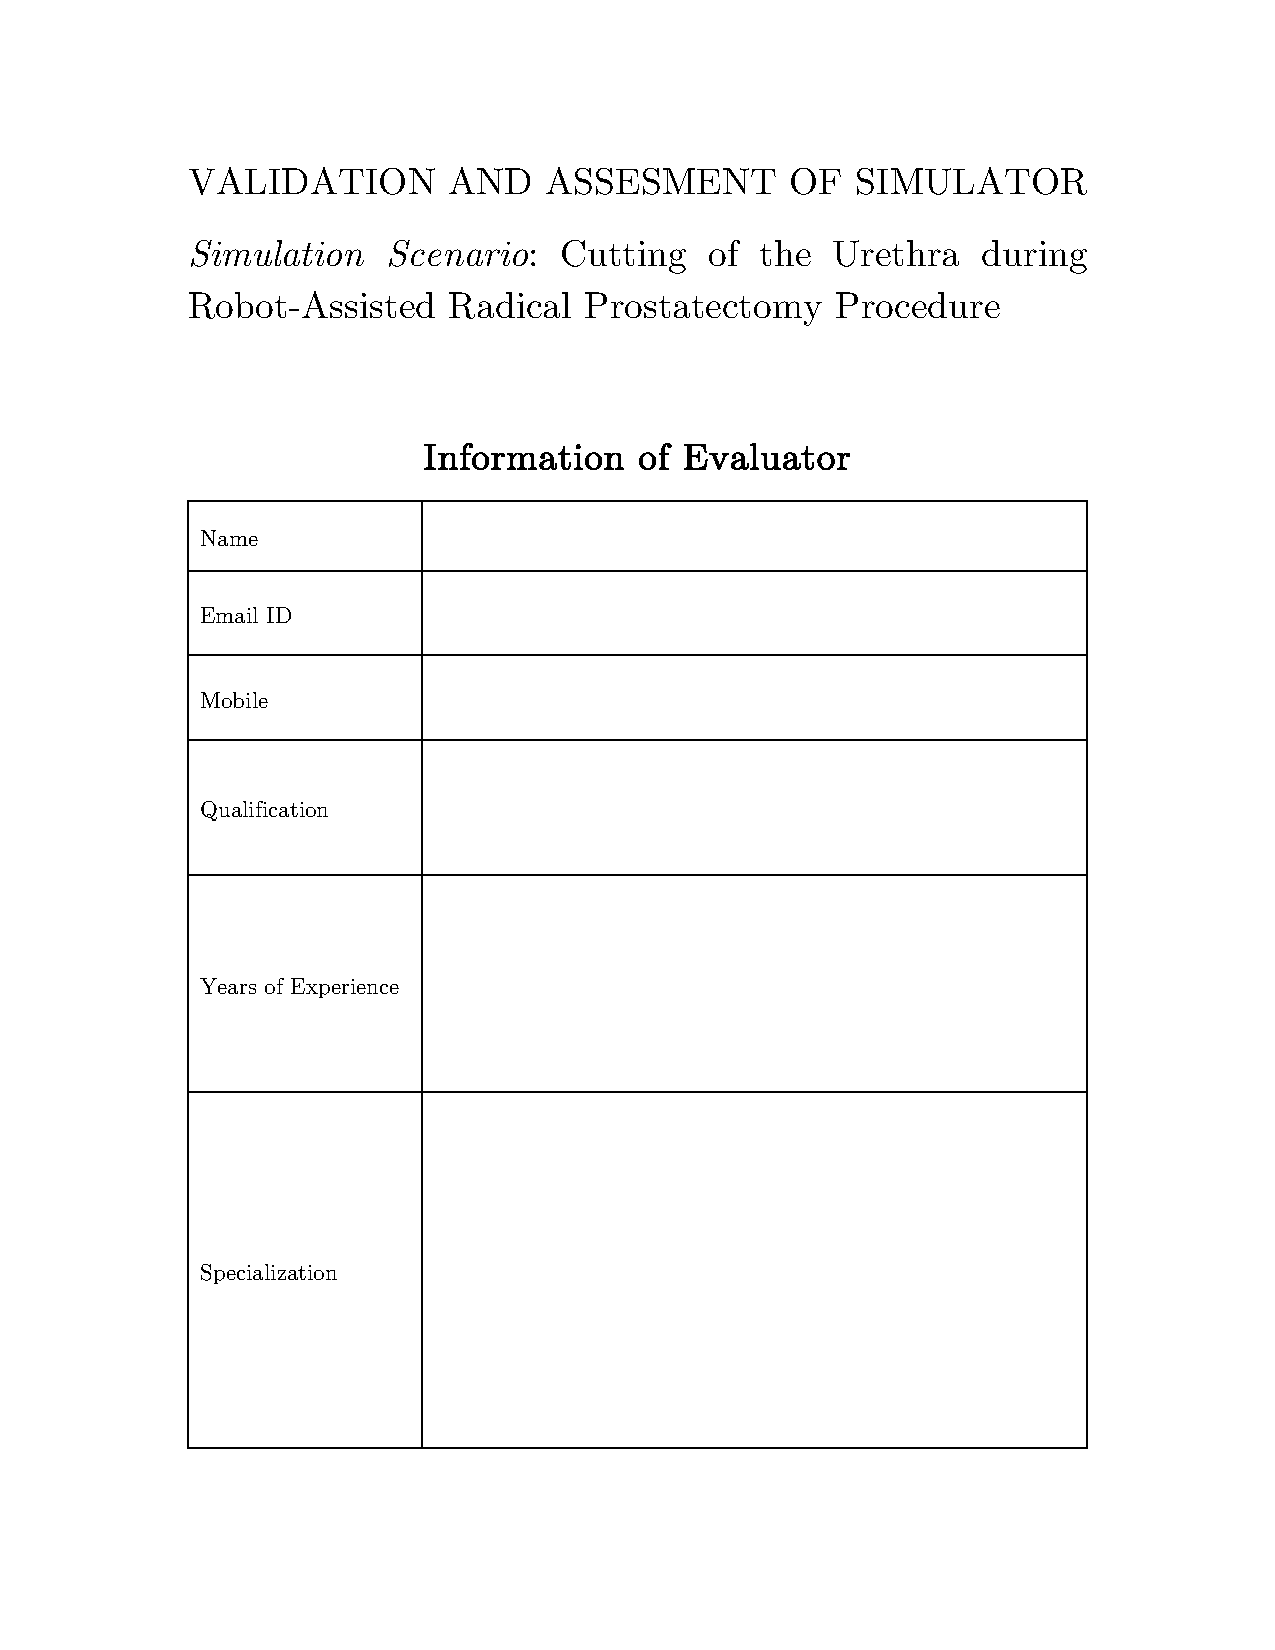
\includepdf[pages=1,pagecommand=\chapter{Evaluation Questionnaire}\label{apn:questionnaire}]{documents/validation/questionnaire.pdf}
%\includepdf[pages=2-,pagecommand={}]{documents/validation/questionnaire.pdf}

\chapter{Individual Contribution}\label{apn:individual_contribution}
\begin{description}[itemsep=1em]
  \item [Abdulla AlAnsari] Co-Lead PI at HMC, has led the team effort inside Qatar. He has supported and guided the overall research, especially the clinical related activities at HMC. He has been actively involved in facilitating activities between different HMC departments. He closely follows-up all project tasks. In particular, he has worked more closely on Aim 5 and 6.
  \item [AbdulRahman AlFayad] worked closely on Aim 1, 4 and 6, mainly development for improving the prototype integration, modeling, and validation. He also worked on the Sofa testing and validations in Aim 2 and 4.
  \item [Ahammed Waseem Palliyali] worked closely on Aim 1, 4 and 6, mainly development for improving the prototype integration, modeling, and validations
  \item [Dinesh Manocha] PI at UNC, participated in all project meetings, and although he contributes to most project tasks, his work focuses on Aim 3. He is supervising an RA and has worked closely on Aim 1, 3, 4 and 5.
  \item [Georges Younes] coordinates the software development efforts. He was mainly focused on Aim 1 and 4, while contributing to all the other aims.
  \item [George Turkkiyyah] Lead-PI at AUB, coordinated research activities between AUB and its partners in Qatar. He has led the team effort at AUB, primarily concerned with the development of discontinuous finite element formulations for tissue cutting, and overall development of the project. He is supervising an RA and has contributed in all project tasks, and more specifically on Aim 1, 2, 4, and 5.
  \item [Gorune Ohannessian] worked closely on Aim 2, mainly algorithms and implementation for simulating cuts in tetrahedral meshes.
  \item [Hawa Hamza]
  \item [Jhasketan Phadan]
  \item [Julien AbiNahed] PI at HMC, has been in charge of overall project coordination/management, mainly of the team in Qatar, and ensures that all HMC tasks are met. He coordinates closely with entire team in Qatar and participates in most project tasks. He has worked on all aims.
  \item [Liang He]
  \item [Nicolas AlHaddad]
  \item [Nikhil Navkar] PI at HMC, co-manages and coordinates technical efforts mainly of team in Qatar and ensures that all HMC tasks are met. Although he contributes on all tasks, he is more focused on Aim 4, 5, and 6.
  \item [Samer Itani]
  \item [Sarra Kharbach]
  \item [Yasmin Halwani]
  \item [Zherong Pan] worked closely on Aim 3, mainly algorithms and implementation for continuous collision detection using bounding volume hierarchies.


  \item [Abdulla Boabed]
  \item [Shaymaa Khalifa]
  \item [Santu Paul]
\end{description}

\chapter{Research Output}\label{apn:research_output}


\backmatter%
